\section{Development Method}

As mentioned earlier this is a learning project and therefore we have been required to use the same development method in our multi project groups. Therefore we have looked into two different methods \textit{XP}(eXtreme Programming) \cite{XP}, and Scrum \cite{SCRUM}, both are agile development methods.
As a part of our courses we have been further introduced to how each method work and how each one they can be implemented in the development process. 

With the knowledge of both XP and Scrum we in the multi project decided to use Scrum (Seen in Figure \vref{fig:ScrumFrameworkFlow}) along with Scrum of Scrums. 

\begin{figure}[ht]
	\centering
		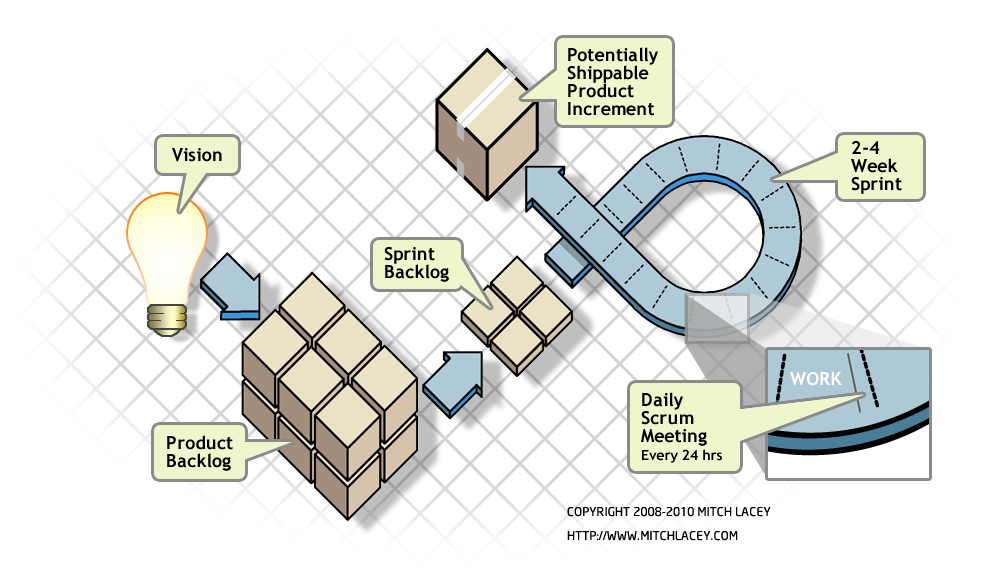
\includegraphics[scale = 0.45]{images/ScrumFrameworkFlow.png}
	\caption{An Overview of the Scrum Framework}
	\label{fig:ScrumFrameworkFlow}
\end{figure}

To enhance our use of Scrum we customized elements of Scrum to fit our project. The changes in the customized version of Scrum, and Scrum of Scrums are:
\begin{itemize}
	\item The sprint length have been shortened to approximately 7 - 14 half days.
	\item Some degree of pair programming have been introduced.
	\item There is no project owner because this is a learning project.
	\item Everyone is attending the Scrum of Scrums meetings.
	\item The Scrum of Scrums meetings are only held once at sprint planning.
\end{itemize}

The benefits from choosing Scrum, and Scrum of Scrums with the customizations are that everyone, at all times, will be able to know what the vision of the project is, and how close every group is to achieving their individual goals of the vision.

As a part of Scum we maintain a close contact with the customers. This helps keep the product backlog up to date and correctly prioritized. The customer are presented with the vision of the project as well as sprint demonstrations of the different incrementation of the product.